\label{sec:methods}
\section{Methods and Materials}

The design and the implementation of the nuclear reactor were carried out using MCNP5.1 run both locally, as well as remotely on servers to verify results. The design was approached in a "bottom-up" fashion. This meant that the reactor's core was designed and tested first. After this, the surrounding material, as well as its geometry, were designed and tested for optimal neutron reflectivity. Finally, the output chamber was added with an FMESH tally running the neutron counts. This approach allowed us to incrementally structure the reactor and catch any errors in their early stages.\\

\subsection{Core}

After considering several variations of breeder reactors, all of which were Thorium based, the element of choice for the core was Uranium-235. Due to safety concerns for real-life implementation, its purity could not be 100\%, however criticality calculations were carried out to understand initial core sizes at this percentage. For a full list of tables of reactivity values, see the results - section \ref{sec:results}.

The approach to determine the core size and composition was the following. Initially, pure Uranium-235 was used. The size of this core was adjusted multiple times to see the impact of the dimensions on the criticality. This impact was observed to be linear, as seen in table.%Table ref here
These first simulations did not account for a shell reflecting neutrons back into the core, nor did it look at the material inside the shell. The values were vague, however, painted the general picture of how large the core should be and how size impacts the criticality.

The next step was to determine how the surrounding material affected the criticality of the core. As seen in table %another ref here,
water had a better impact on the core's ability to fission than vacuum. This was contrary to our initial beliefs, as we thought water would absorb the neutrons and dampen the reactions. Looking at the values, one can see that water actually improved the fission reactions.

Through these initial simulations, the core was to be surrounded in water for optimum criticality. The next step was to vary the material of the shell, against which the neutrons would reflect. A thickness of $5cm$ was arbitrarily chosen to make sure the particles would not escape the chamber. Between zirconium and graphite, the latter performed better in reflecting the neutrons and sustaining the nuclear reactions. This is seen by results of our simulations in tables %two refs here for zirconium and graphite shells

The final in the core design was to look at the enrichment percentage. The issue with 100\% U-235 composition is that it is extremely difficult to achieve, as well as the fact that that level is weapons-grade. Low-power reactors usually have enrichment percentages of 3\%-7\%, while something with more power could have a level of around 20\%. The rest of the material was to be U-238, which is found in nature, but with a U-235 percentage composition of 0.07\%. Seen in tables %ref them again
one can see the various size and composition configurations looked at to achieve a k-coefficient value of 1. The final core design was settled to be a cube, side length of $l=30cm$. The U-235 enrichment level would be 15\%, yielding a k-coefficient of $k=1.06625$.
\subsection{Shell}

The surrounding shell and its geometry have several purposes in the reactor:
\begin{enumerate}
	\item Neutron reflection. The neutrons that are emitted from the core need to not be lost after one interaction. As a result, the surrounding shell's geometry was optimized to increase reflectivity of particles back into the core. The thermal neutrons will reflect off of the walls and be directed towards the core to trigger further fissions.
	\item Thermal regulation. Any heat given off by the fission reactions needs to be transported out of the system to control the temperature. This is outside the scope of the project, however, some discussion is given in section \ref{sec:future}.
	\item Particle interaction. This is a middle ground between the previous two purposes. The material that the core is submerged in plays an important role in particle interaction. Materials looked at were water, graphite and vacuum.
\end{enumerate}

\subsubsection{Neutron reflection}

An already existing example of reflection was taken into account when looking at the shell's neutron reflection capabilities - a parabolic dish. A ray diagram of how a parabolic reflector works can be seen in figure \ref{fig:parabola}.

\begin{figure}[!htbp]
\caption{Parabolic reflector.}
\label{fig:parabola}
\centering
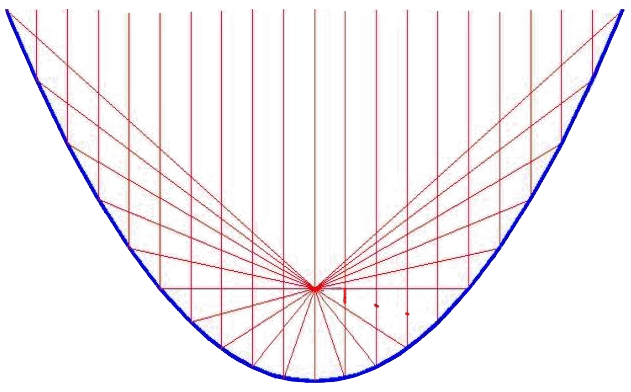
\includegraphics[width=0.75\textwidth]{parabola.png}
\end{figure}

From this, a circular design of the shell was implemented for initial simulations, with the reactor core in the middle. However, looking at the structure presented in figure \ref{fig:structure}, a problem arose with neutron direction.

\begin{figure}[!htbp]
\caption{Core and shell structures.}
\label{fig:structure}
\centering
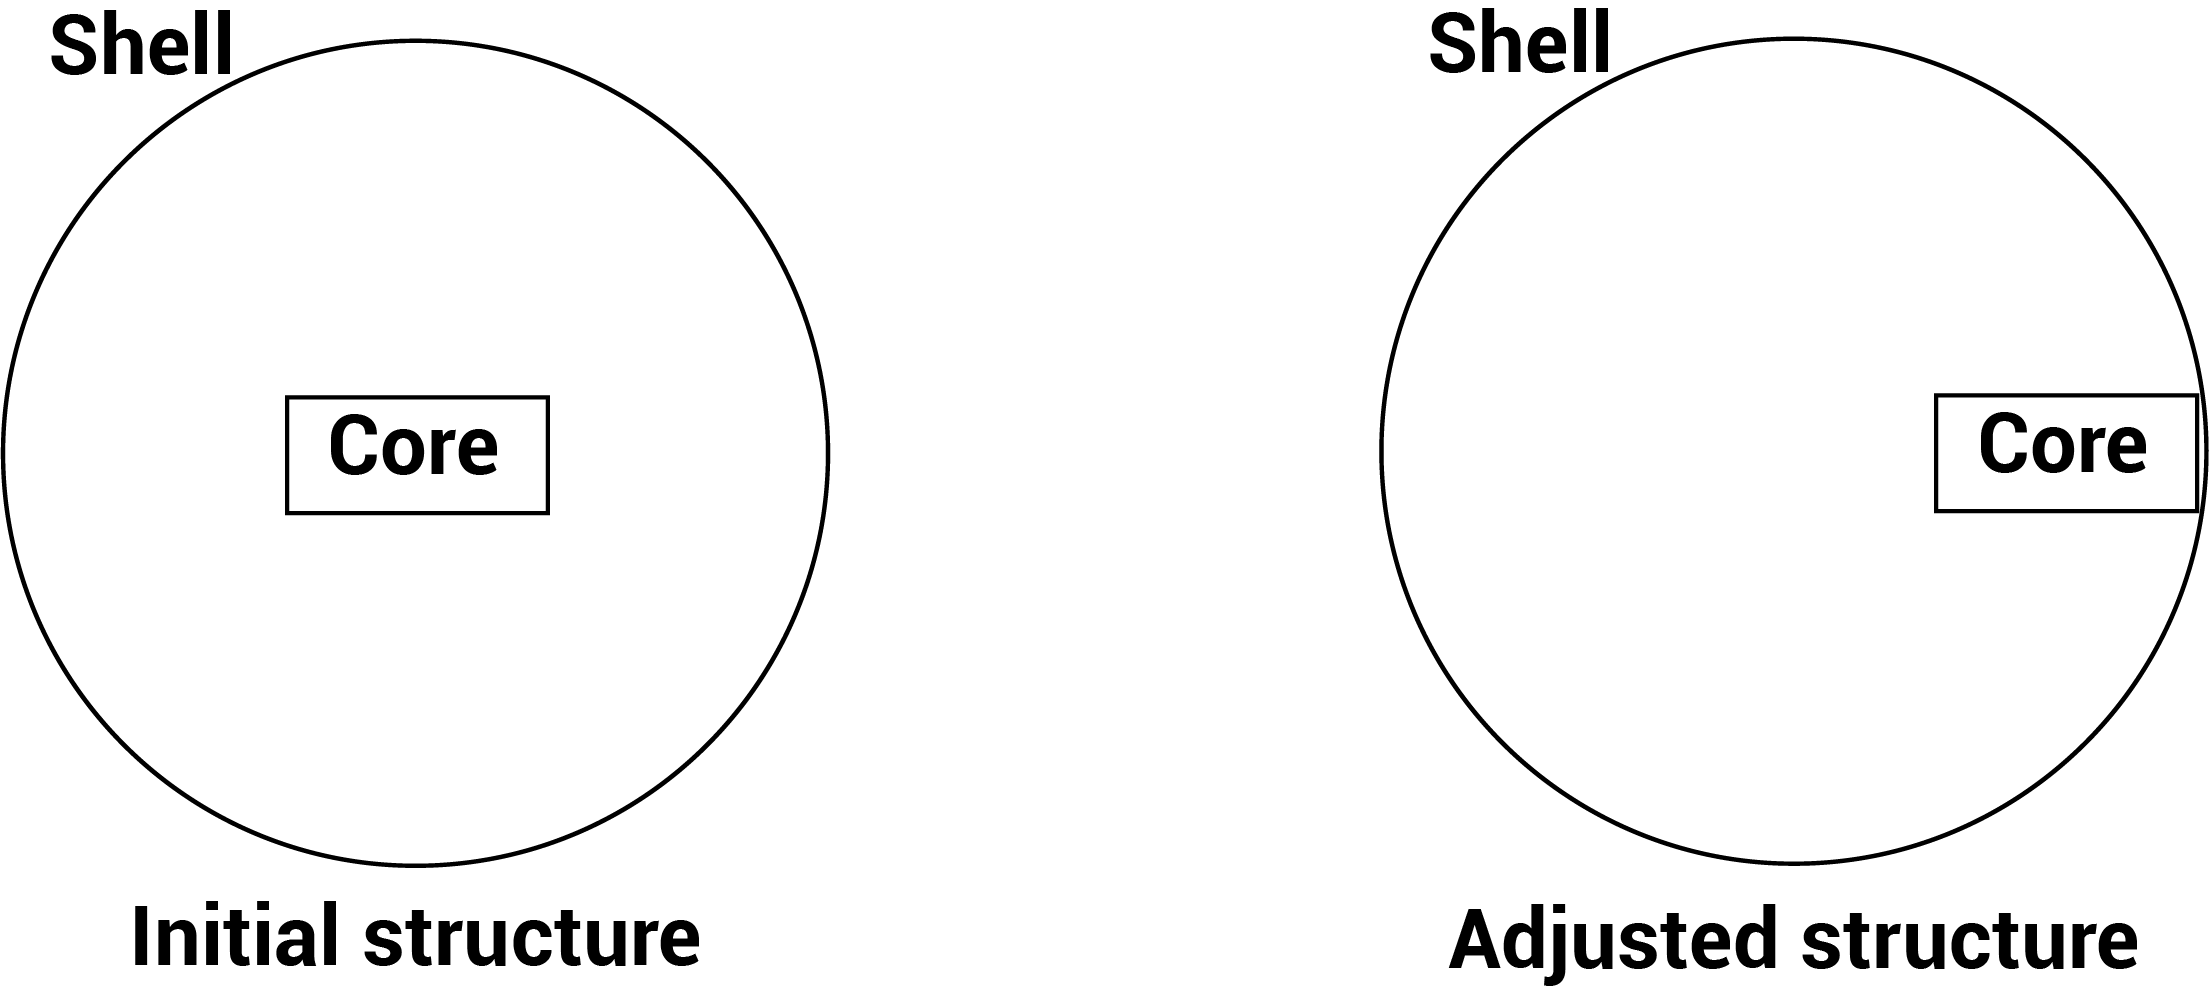
\includegraphics[width=0.75\textwidth]{structure.png}
\end{figure}

Neutrons that are to be used in research would be extremely difficult to direct towards an opening. Whatever directing structure that had to be added to the geometry would interfere with the parabolic reflective properties. As a result, a decision was made to move the core to one edge of the shell, seen under "Adjusted structure" in figure \ref{fig:structure}.

\subsubsection{Particle interaction}

Several materials were looked at with which to fill the shell around the core. These were water, graphite and vacuum. Looking at the criticality results in section \ref{sec:results},
%ref the specific tables
using water enabled a criticality coefficient of $k\approx 1$. This meant that the core was perfectly critical - with little chances of creating a runaway chain reaction or the fission reactions dying out. Vacuum did not interact with the neutrons at all, which may have created issues later on with sustained reactions. Graphite, on the other hand
%I need to run one more test here

\subsection{Chamber}

With the core shifted to the side of the enclosing shell, it was now possible to add the neutron chamber on that very side. One side of the core's structure would be directly exposed to the chamber. As a result, the neutrons produced on that side would be emitted directly for flux calculations and use. The other 5 sides of the rectangular core structure would be fueling the fission reactions through the emission and reflection of thermal neutrons within the shell itself. From the criticality results, seen in section \ref{sec:results}, the side length of the core was taken to be $l=30cm$ in each direction. From this we see that the core is actually a cube. As a result, the cross section of the chamber is 30x30cm in order to capture all particles emitted.

\begin{figure}[!htbp]
\caption{Shell, core, chamber structure.}
\label{fig:chamber}
\centering
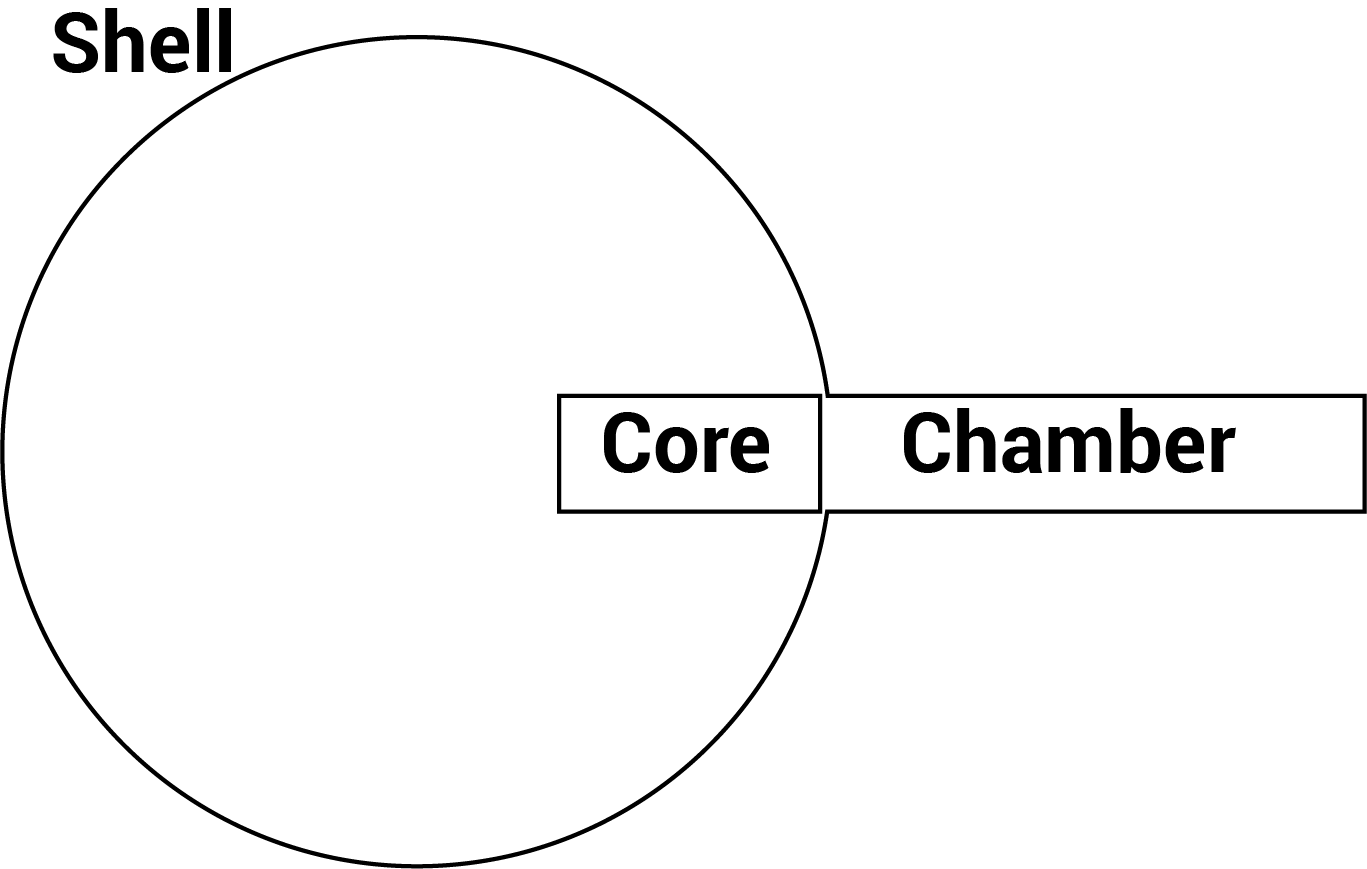
\includegraphics[width=0.75\textwidth]{chamber.png}
\end{figure}

The placement of the core reduces particle leak, however, due to the nature of the geometry (cube placed against a spherical surface), some neutrons may leak back into the shell. The flux lost due to this is negligible since the returned neutrons will fuel further fission reactions after being reflected back into the core by the shell. The structure of the shell, core and neutron chamber can be seen in figure \ref{fig:chamber}. Naturally, the neutron flux tally will be carried out in the chamber.

\subsection{Tally}

